\documentclass[conference]{IEEEtran}
\usepackage{amsmath,booktabs,longtable,graphicx}
\usepackage{pgfplots}
\pgfplotsset{compat=1.17}
\usepackage[hidelinks]{hyperref}
\begin{document}
\title{K-Nearest-Neighbor Classification with CUDA and MPI}
\author{\IEEEauthorblockN{Rahat Rizvi Rahman}
\IEEEauthorblockA{Department of Computer Science\\Virginia Commonwealth University\\Richmond, USA\\rahmanr12@vcu.edu}}
\maketitle
\begin{abstract}
This report evaluates global-memory and shared-memory CUDA implementations of the KNN classifier and an MPI+CUDA extension. The same datasets and classification rules from Assignment 1 are retained. Archived evidence contains 342 completed benchmark runs across Maple, Athena A100 and H100 GPU nodes, and an Athena CPU node. Every measured prediction array matches the serial reference. On the large dataset, the best observed single-GPU configurations achieve same-sweep serial speedups of 21.44 on Maple, approximately 37.8 on the A100, and approximately 34.4 on the H100. These speedups have different host CPU baselines. Shared-memory tiling reduces runtime relative to the global kernel in every tested configuration of the paired Athena sweeps. MPI+CUDA correctness is verified on up to four H100 GPUs in one node and two V100 nodes, but repeated multi-GPU timing results are not available. This report distinguishes measured results, correctness-only evidence, and outstanding experiments.
\end{abstract}
\begin{IEEEkeywords}KNN, CUDA, shared memory, MPI, performance measurement\end{IEEEkeywords}

\section{Introduction}
K-nearest-neighbor classification compares a test query with all training instances, retains the closest $k$ neighbors, and predicts their most frequent label. The independent test queries provide a direct decomposition for parallel execution. Assignment 2 extends the Assignment 1 CPU implementations using CUDA and MPI+CUDA. The design uses the supplied lectures on thread indexing, memory transfers, memory access, shared-memory tiling, and multi-GPU coordination \cite{cuda8,cuda9,cuda10,cuda13,mpi6}.

The experimental questions are whether GPU classification reduces complete classification time, whether reusing training rows through shared memory improves the global-memory baseline, and how block size affects the observed means. A separate MPI implementation establishes correctness across devices and nodes. Repeated multi-GPU scaling remains an uncompleted experiment in the evidence available for this report.

\textbf{Evidence cutoff.} This report uses results committed through \texttt{7ef8264}, with experiment records dated October 22--23, 2026. It is a report of available evidence as of that snapshot. A queued job's status is not a live observation and may change after the snapshot. The missing Maple shared-memory measurements and timed MPI+CUDA sweep are explicitly identified below.

\section{Methodology}
\subsection{Datasets and serial reference}
The original ARFF datasets and parser are reused without preprocessing changes. The class column is excluded from distance computation. All measured experiments use $k=3$, float accumulation in the original feature order, and Euclidean distance including the square root.
\begin{table}[t]\centering
\caption{Dataset sizes and reference accuracy. Features exclude the class label.}\label{tab:data}
\small\begin{tabular}{lrrrr}\toprule
Dataset & Train & Test & Features & Accuracy (\%)\\\midrule
Small & 1,184 & 160 & 7 & 85.000000\\
Medium & 14,708 & 740 & 11 & 27.567568\\
Large & 61,606 & 3,436 & 11 & 99.476135\\\bottomrule
\end{tabular}\end{table}
Training rows are scanned in their original order. A candidate replaces an entry only when its distance is strictly smaller, preserving earlier training rows in equal-distance ties. A tied class vote selects the smallest class index. The medium dataset's relatively low accuracy is the unchanged reference outcome, not an introduced GPU discrepancy. With insertion-based selection, work is approximately $O(N_qN_t(d+k))$ for $N_q$ queries, $N_t$ training rows, and $d$ features.

\subsection{Global-memory CUDA kernel}
One CUDA thread handles one test query. Its index follows the lecture grid/block mapping. The thread scans all training rows, maintains a sorted top-$k$ candidate list, counts class votes, and writes one prediction. Candidate distances, labels, and vote counters occupy distinct per-query slices of global-memory workspace. They are private by ownership, not by memory placement. The host flattens the matrices, allocates device buffers, transfers inputs, launches the kernel, and retrieves predictions. Out-of-range query threads return without doing work.

\subsection{Shared-memory CUDA kernel}
The second kernel retains the query-to-thread mapping and candidate-selection helpers. A block cooperatively loads a tile of training rows into dynamic shared memory. Adjacent threads load adjacent flattened elements using a stride equal to block size. After a barrier, active query threads scan the tile in training-row order; a second barrier precedes replacement of the tile. Inactive threads in a partial query block still participate in both barriers. Partial training tiles load and scan only valid rows.

The tile is fixed at 256 training rows. Including the class column, the small dataset requires 8,192 shared bytes per block and the other datasets require 12,288 bytes. Only training-row storage changes; candidate lists and votes remain in global memory. The approach follows the shared-memory reuse examples in Lecture 10 \cite{cuda10}. Tile size is not swept, so results do not identify its optimum.

\subsection{MPI+CUDA decomposition}
Each MPI rank uses one allocated GPU. Node-local rank and visible device count determine device selection, and a UUID check rejects accidental sharing of the same GPU by multiple ranks. Rank $r$ of $P$ handles the half-open test interval
\begin{equation}
[\lfloor rN_q/P\rfloor,\ \lfloor(r+1)N_q/P\rfloor).
\end{equation}
Each rank retains the full training matrix and transfers its own query range to its GPU. Both CUDA kernels are shared with the single-GPU program. Local predictions return to host memory and \texttt{MPI\_Gatherv} restores the global query order on rank zero. Empty ranges skip the GPU launch but participate in communication. Exceptions abort the MPI job to prevent other ranks waiting indefinitely. This adapts the supplied multi-host CUDA example and MPI material \cite{cuda13,mpi6}.

\subsection{CPU comparisons and timing}
The serial, pthreads, OpenMP, and CPU MPI programs retain the same query decomposition and decision rule. CPU parallel worker counts are 1, 2, 4, 8, and 16. The CPU MPI study uses one node. Each configuration is measured three times, using a fresh process with no explicit warm-up. CUDA block sizes are 64, 128, and 256. Both strategies are tested in the paired A100 and H100 sweeps.

The primary timer measures classification after ARFF parsing. It includes matrix flattening, workspace allocation, GPU transfers, kernel execution, prediction retrieval, and workspace cleanup. Parsing, validation, device discovery, accuracy calculation, and prediction-file output are excluded. Returned predictions remain allocated at the end of the timer. Thus ``end-to-end'' refers to classification, not whole-process or file-to-output elapsed time. CPU timers use the corresponding classification boundary. MPI timers exclude MPI initialization and launcher overhead, start after a barrier, include result gathering, and report the maximum rank duration. GPU kernel time uses synchronized CUDA events \cite{cuda9}.

For each single-GPU sweep, speedup is
\begin{equation}
S_{\mathrm{serial}}=\frac{\overline{T}_{\mathrm{serial,same\ sweep}}}{\overline{T}_{\mathrm{GPU,classification}}}.
\end{equation}
Kernel-only times are never substituted in the denominator. For a timed MPI+CUDA sweep, the intended definitions are $S_g=\overline{T}_{\mathrm{MPI+CUDA}}(1)/\overline{T}_{\mathrm{MPI+CUDA}}(g)$ and $E_g=S_g/g$. These values are not computed without repeated scaling measurements. CPU relative efficiency uses the same CPU program at one worker as its baseline, divided by worker count.

\subsection{Environment and reproducibility}
\begin{table*}[t]\centering
\caption{Experimental environments. Times from different rows are never pooled.}\label{tab:hardware}
\small\begin{tabular}{llll}\toprule
Platform/node & GPU & Host CPU & Evidence\\\midrule
Maple & GTX 1080 Ti, 11 GiB & Xeon E5-2690 v4 & Global baseline\\
Athena 521 & A100-SXM4-80GB & AMD EPYC 7763 & Global baseline and paired sweep\\
Athena 533 & H100 80GB HBM3 & Xeon Platinum 8462Y+ & Paired sweep; 1--2 GPU verification\\
Athena 531 & H100 80GB HBM3 & Xeon Platinum 8480CL & 1--4 GPU verification\\
Athena 513/514 & V100 & Not used for CPU timing comparisons & Two-node correctness only\\
Athena 201 & None & AMD EPYC 7742 & CPU comparison, 16 allocated CPUs\\\bottomrule
\end{tabular}\end{table*}
All computation was scheduled through Slurm. GPU sweeps requested one GPU and one CPU. The CPU sweep used 16 allocated CPUs on a nonexclusive node without explicit thread pinning. CUDA toolkit 12.3.107 and GCC 11.4 were used for GPU builds; CPU comparison used GCC 11.4.1 and Open MPI 4.1.6. CPU flags include \texttt{-O2 -std=c++11 -ffp-contract=off}, and CUDA flags include \texttt{-O2 -std=c++11 --fmad=false}. A100, H100, and V100 builds target \texttt{sm\_80}, \texttt{sm\_90}, and \texttt{sm\_70}; the original Maple build did not specify an architecture flag. Fast math is not enabled.

The source snapshots and patches identify the code used by each sweep. The initial A100 baseline predates the shared-helper refactor; its measurements are retained separately from the paired comparison. Compile jobs targeting different GPU architectures must run sequentially when using a shared checkout. An earlier concurrent H100/V100 build was followed by a missing-kernel-image failure, consistent with the binary being replaced. A sequential rerun passed.

\section{Results}
\subsection{Correctness and completed measurements}
All 342 measured prediction arrays match their serial references byte for byte. The evidence comprises 36 Maple baseline runs, 36 initial A100 baseline runs, 63 paired A100 runs, 63 paired H100 runs, and 144 CPU runs. Every group has three repetitions. Archive checksums and all 7,025 manifest entries were checked; CSV values match individual logs, and summary statistics and label-based accuracy were recomputed. The appendix gives every individual classification time and mean.

Synthetic verification exercises neighbor ties, vote ties, runtime $k$, invalid arguments, partial query blocks, and partial training tiles. MPI tests add uneven and empty rank ranges, rank/device mapping, and injected-rank failure. Dedicated MPI dataset comparisons were independently checked for full prediction equality, distinct host/device assignments, and complete query coverage.

\begin{table}[t]
\centering\caption{Lowest observed mean GPU classification time per dataset. Speedup uses serial from the same sweep.}\label{tab:best}
\small\setlength{\tabcolsep}{3pt}\begin{tabular}{lllrrr}\toprule
GPU & Data & Kernel & Block & ms & Speedup \\
\midrule
GTX 1080 Ti & small & global & 128 & 2.699 & 0.67 \\
GTX 1080 Ti & medium & global & 64 & 29.941 & 4.17 \\
GTX 1080 Ti & large & global & 128 & 111.926 & 21.44 \\
A100 & small & shared & 256 & 1.488 & 0.93 \\
A100 & medium & shared & 128 & 13.016 & 7.96 \\
A100 & large & shared & 64 & 52.563 & 37.81 \\
H100 & small & shared & 128 & 1.174 & 0.89 \\
H100 & medium & shared & 128 & 10.261 & 7.39 \\
H100 & large & shared & 128 & 42.479 & 34.37 \\
\bottomrule\end{tabular}
\end{table}

\begin{figure}[t]
\centering
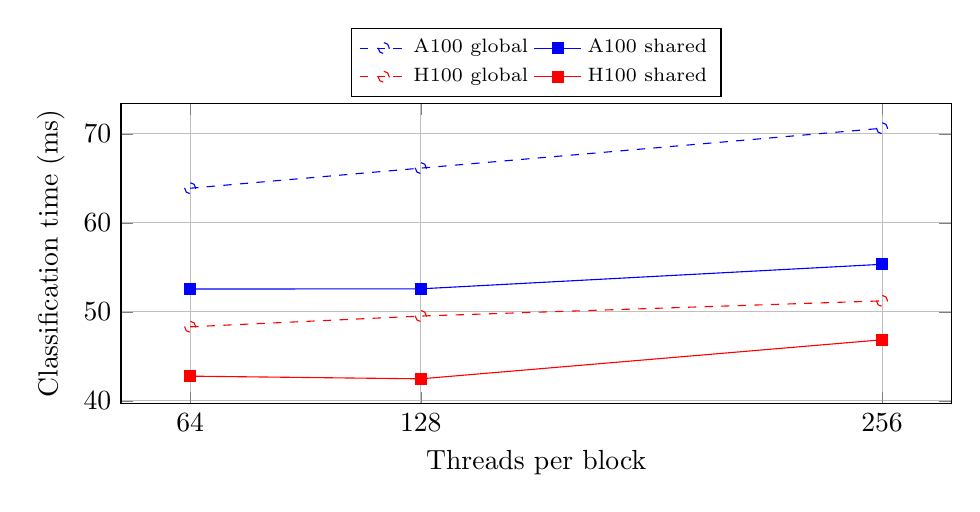
\begin{tikzpicture}
\begin{axis}[width=\columnwidth,height=5.4cm,xlabel={Threads per block},ylabel={Classification time (ms)},xtick={64,128,256},legend style={font=\scriptsize,at={(0.5,1.02)},anchor=south,legend columns=2},grid=major]
\addplot[blue,dashed,mark=o] coordinates {(64,63.889098) (128,66.14855) (256,70.62373533333333)};
\addlegendentry{A100 global}
\addplot[blue,solid,mark=square*] coordinates {(64,52.562508666666666) (128,52.589258666666666) (256,55.343317666666664)};
\addlegendentry{A100 shared}
\addplot[red,dashed,mark=o] coordinates {(64,48.321567333333334) (128,49.530923666666666) (256,51.233959)};
\addlegendentry{H100 global}
\addplot[red,solid,mark=square*] coordinates {(64,42.779333333333334) (128,42.47874233333333) (256,46.863927000000004)};
\addlegendentry{H100 shared}
\end{axis}\end{tikzpicture}
\caption{Large-dataset block-size experiment, three-run means from the paired sweeps. Hardware differs between A100 and H100.}\label{fig:gpu}
\end{figure}

\subsection{Single-GPU configurations}
Table~\ref{tab:best} reports the lowest observed means, and Fig.~\ref{fig:gpu} compares block sizes on the large dataset. The Maple global kernel reaches 21.44 times its own serial baseline on large, but the small dataset is slower on the GPU. The paired A100 and H100 sweeps contain both strategies at all block sizes on all datasets. Within each sweep, shared-memory classification is faster than the global kernel at every matched block size. Ratios of global to shared time range approximately from 1.10 to 1.28 on A100 and 1.02 to 1.17 on H100.

At block 128 on large, shared-memory classification takes approximately 52.589 ms on A100 and 42.479 ms on H100. Their host serial means differ, approximately 1987.5 ms and 1459.9 ms respectively, so their speedup values do not isolate GPU hardware differences. The best observed block size also depends on dataset and device. All tested small-dataset GPU configurations remain slower than the same-sweep serial reference.

\begin{table}[t]
\centering\caption{CPU configurations with lowest observed mean, EPYC 7742. Range spans three runs.}\label{tab:cpu}
\small\setlength{\tabcolsep}{3pt}\begin{tabular}{llrrrr}\toprule
Data & Program & Workers & Mean & Min & Max \\
\midrule
small & serial & 1 & 2.839 & 2.827 & 2.860 \\
small & pthreads & 8 & 1.559 & 1.246 & 1.830 \\
small & openmp & 4 & 1.354 & 1.303 & 1.431 \\
small & mpi & 16 & 0.476 & 0.356 & 0.579 \\
medium & serial & 1 & 198.469 & 198.331 & 198.654 \\
medium & pthreads & 8 & 34.326 & 28.402 & 45.595 \\
medium & openmp & 8 & 29.403 & 29.094 & 29.780 \\
medium & mpi & 16 & 18.041 & 17.749 & 18.543 \\
large & serial & 1 & 2594.672 & 2313.991 & 3153.929 \\
large & pthreads & 16 & 465.712 & 405.054 & 548.117 \\
large & openmp & 16 & 535.541 & 527.790 & 541.068 \\
large & mpi & 16 & 241.172 & 228.142 & 262.670 \\
\bottomrule\end{tabular}
\end{table}

\begin{figure}[t]\centering
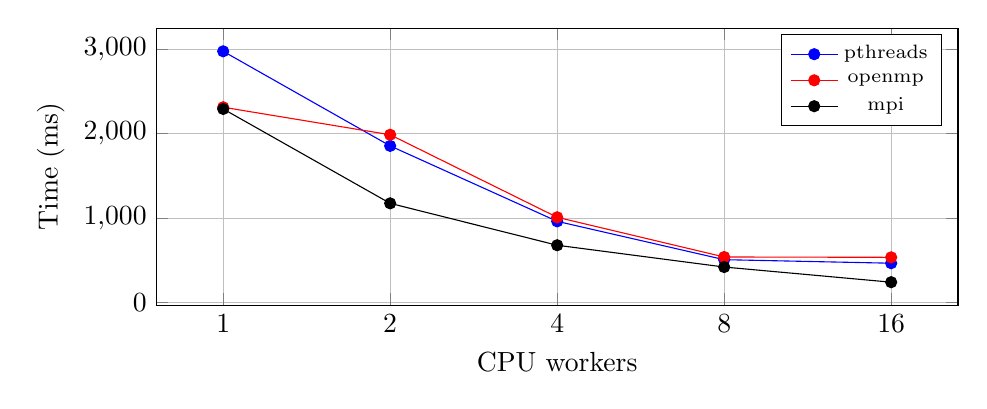
\begin{tikzpicture}\begin{axis}[width=0.97\columnwidth,height=5.1cm,xlabel={CPU workers},ylabel={Time (ms)},xmode=log,log basis x=2,xtick={1,2,4,8,16},xticklabels={1,2,4,8,16},legend style={font=\scriptsize},grid=major]
\addplot[blue,mark=*] coordinates {(1,2974.2846956666667) (2,1854.6393073333334) (4,961.5561986666667) (8,507.641633) (16,465.71177266666666)};\addlegendentry{pthreads}
\addplot[red,mark=*] coordinates {(1,2312.296442) (2,1986.5161413333333) (4,1009.533049) (8,539.393819) (16,535.5408663333333)};\addlegendentry{openmp}
\addplot[black,mark=*] coordinates {(1,2291.9239063333334) (2,1174.5926776666668) (4,678.410175) (8,420.45948100000004) (16,241.17197033333335)};\addlegendentry{mpi}
\end{axis}\end{tikzpicture}
\caption{Large-dataset CPU classification times on Athena's EPYC 7742 node. Three-run means are shown; individual values in the appendix expose run-to-run variation.}\label{fig:cpu}
\end{figure}

\begin{table}[t]
\centering\caption{Cross-platform CPU/GPU time ratios. CPU uses EPYC 7742 (16 workers for parallel programs); GPU uses H100 with Xeon 8462Y+ host. Ratios are not same-machine speedups.}\label{tab:cross}
\small\setlength{\tabcolsep}{3pt}\begin{tabular}{lrrrrr}\toprule
Data & GPU ms & Serial & Pthreads & OpenMP & MPI \\
\midrule
small & 1.174 & 2.42 & 2.25 & 54.97 & 0.41 \\
medium & 10.261 & 19.34 & 3.93 & 7.64 & 1.76 \\
large & 42.479 & 61.08 & 10.96 & 12.61 & 5.68 \\
\bottomrule\end{tabular}
\end{table}

\subsection{CPU and GPU comparisons}
Table~\ref{tab:cpu} reports the fastest observed configuration for each CPU program and dataset, including its three-run range. Fig.~\ref{fig:cpu} shows large-dataset CPU scaling. At 16 MPI ranks, large takes 241.172 ms versus a serial mean of 2594.672 ms on the CPU node, a speedup of 10.76. The corresponding H100 shared-kernel mean is 42.479 ms.

Table~\ref{tab:cross} explicitly compares the separate 16-CPU allocation with one H100. It includes serial, pthreads, OpenMP, and CPU MPI. These are cross-platform time ratios, not controlled same-host CPU/GPU speedups. GPU performance is not uniformly better; the small-dataset CPU MPI mean at 16 ranks is approximately 0.476 ms, below the H100 classification mean of 1.174 ms.

\subsection{MPI+CUDA correctness and missing timings}
\begin{table}[t]\centering
\caption{Completed MPI+CUDA dataset verification. Counts cover three datasets, both kernels, and three block sizes per layout. These are correctness runs, not repeated timing experiments.}\label{tab:mpi}
\small\begin{tabular}{llll}\toprule
Job & GPU & Node/rank layouts & Matches\\\midrule
3382992 & H100 & 1 node, 1/2 ranks & 36/36\\
3382997 & H100 & 1 node, 1/2/3/4 ranks & 72/72\\
3382990 & V100 & 1/2 nodes, 1 GPU/node & 36/36\\\bottomrule
\end{tabular}\end{table}
Multi-GPU and two-node allocations were obtained for verification (Table~\ref{tab:mpi}). They establish functional correctness of the delivered MPI+CUDA implementation. Their unrepeated timing prints do not establish scaling or efficiency and are not used as benchmark rows.

The timed H100 scaling job, 3383610, was submitted to request four GPUs on one node and test 1, 2, and 4 GPUs, all datasets, and three repetitions. The saved handoff reports it still queued at the October 23 evidence cutoff because a suitable allocation was unavailable. No benchmark output for it is included. Submission history is archived, but a raw current queue/accounting snapshot for this pending job is absent from the supplied bundle. Its current state must therefore be refreshed before final submission. No multi-GPU speedup or efficiency is reported.

\section{Analysis}
Shared-memory tiling permits each block to reuse training data after cooperative loading, consistent with the lecture's reuse argument. The measured reduction in classification time supports this strategy for the tested configurations. Without profiling, however, the experiments do not isolate memory traffic, cache behavior, or occupancy as the cause. Synchronization overhead and global-memory candidate storage remain part of the implementation.

Available query parallelism is limited. The small dataset has only 160 queries, which produces two blocks at block size 128. The large dataset produces 27 such blocks from 3436 queries. Splitting queries over more GPUs reduces the queries on each GPU while every query still scans the full training set. This makes weak scaling gains plausible, but only the pending repeated benchmark can establish the actual multi-GPU trend. A verification kernel time is not substituted for that experiment.

Fixed classification overhead also matters. On H100, large/shared/block-128 spends approximately 35 ms in its kernel versus 42.479 ms in the complete classification region. The gap includes transfers, allocation, and other host/device work, but the experiments do not separately time each component. This is why kernel-only speedup would exaggerate the observed benefit.

CPU scaling improves clearly through several worker counts, but the means and variation must be read together. On large, pthreads improves from 507.642 ms at eight threads to 465.712 ms at sixteen, while OpenMP changes only from 539.394 to 535.541 ms. On medium both slow down at sixteen. Lack of pinning, scheduling, and shared-node activity are possible contributors, not measured explanations. Serial large on the CPU node ranges from 2313.991 to 3153.929 ms, so its mean-based speedups carry substantial uncertainty.

\subsection{Resource and coverage limitations}
The missing evidence has specific boundaries. Maple has only the original global-memory sweep; the shared-memory implementation still needs verification and a paired global/shared benchmark there. Athena has complete single-GPU paired measurements and CPU comparisons, but no completed repeated multi-GPU or multi-node timing study in the supplied evidence.

An earlier four-A100 request, 3382607, was cancelled after the submission history records more than 18 hours pending. H100 launch attempts involving \texttt{athena534} also failed with Slurm/PMIx communication and TRES errors. V100 two-node verification subsequently passed, so these failures do not show that all multi-node execution on Athena is unavailable. Other failed attempts involved a corrected launcher-template bug and the suspected build collision. These software failures are distinguished from allocation delays.

Only three repetitions, three block sizes, and one tile size were tested. No randomization, warm-up study, or profiler analysis was performed. No confidence interval or universally optimal configuration is claimed. The A100 global baseline and paired sweep differ by several percent on large and remain separate experiments. Hardware differences preclude pooling results across Maple, GPU nodes, and the CPU comparison node. Historical Assignment 1 timings used different flags and timer precision and are excluded.

\section{Conclusion}
The completed evidence establishes correct single-GPU CUDA classification for both kernels on Athena and for the global baseline on Maple, plus MPI+CUDA correctness across up to four GPUs and two nodes. Shared-memory training tiles improve the tested Athena configurations, and medium and large datasets benefit from GPU classification relative to their same-sweep serial baselines. The small dataset does not show this benefit.

The current report does not claim completion of the repeated multi-GPU scaling requirement. The remaining work is the Maple shared-memory sweep and the queued Athena timing experiment, followed by an updated report if results arrive. If the timed allocation remains unavailable at submission, retain this explicit limitation and a dated queue/accounting snapshot. Resource documentation explains missing measurements but does not replace them.

\begin{thebibliography}{6}
\bibitem{cuda8} CMSC 603 lecture materials, ``8. Introduction to CUDA,'' pp. 9--16, supplied course PDF and vector-add example.
\bibitem{cuda9} CMSC 603 lecture materials, ``9. CUDA memory access pattern,'' pp. 2--11, supplied course PDF and matrix-add example.
\bibitem{cuda10} CMSC 603 lecture materials, ``10. CUDA shared memory,'' pp. 2--10, supplied course PDF and tiled matrix multiplication examples.
\bibitem{cuda13} CMSC 603 lecture materials, ``13. CUDA asynchronous streams and multi-GPU,'' pp. 17--25, and supplied \texttt{vectorAdd\_multihost\_multiGPU.cu}.
\bibitem{mpi6} CMSC 603 lecture materials, ``6. MPI,'' supplied slides and collective communication examples.
\bibitem{slurm2} CMSC 603 lecture materials, ``2. Slurm for HPC clusters,'' supplied course PDF.
\end{thebibliography}

\clearpage\onecolumn
\appendices
\section{Individual Measurements and Averages}
Every row contains three independent process invocations. Classification times and kernel means are in milliseconds. GPU speedup uses the serial mean from that same sweep. CPU speedup uses the CPU-node serial mean; CPU efficiency uses the same parallel program at one worker divided by worker count. Kernel means are unavailable for serial rows. Missing experiments are omitted rather than filled with zeros or verification timings. Machine and sweep labels must remain attached to each table.
\subsection{Maple GTX 1080 Ti, global baseline}
\small
\begin{longtable}{lllrrrrrr}
\caption{Maple GTX 1080 Ti, global baseline. Individual classification times and means in ms. Three repetitions per row.}\\
\toprule
Data & Kernel & Block & Run 1 & Run 2 & Run 3 & Mean & Kernel mean & Speedup \\
\midrule\endfirsthead
\toprule
Data & Kernel & Block & Run 1 & Run 2 & Run 3 & Mean & Kernel mean & Speedup \\
\midrule\endhead
\bottomrule\endfoot
small & serial & 0 & 1.812124 & 1.839452 & 1.792599 & 1.814725 & -- & 1.0000 \\
small & global & 64 & 2.766211 & 2.759699 & 2.700355 & 2.742088 & 2.295819 & 0.6618 \\
small & global & 128 & 2.691262 & 2.693923 & 2.710614 & 2.698600 & 2.259627 & 0.6725 \\
small & global & 256 & 2.764347 & 2.763593 & 2.790888 & 2.772943 & 2.323435 & 0.6544 \\
medium & serial & 0 & 124.944742 & 124.954892 & 124.975649 & 124.958428 & -- & 1.0000 \\
medium & global & 64 & 29.990609 & 29.926695 & 29.905640 & 29.940981 & 27.124362 & 4.1735 \\
medium & global & 128 & 30.171638 & 30.044490 & 30.092245 & 30.102791 & 27.298816 & 4.1511 \\
medium & global & 256 & 32.677940 & 32.691904 & 32.488903 & 32.619582 & 29.794923 & 3.8308 \\
large & serial & 0 & 2399.853160 & 2399.197048 & 2400.790090 & 2399.946766 & -- & 1.0000 \\
large & global & 64 & 138.463878 & 126.104135 & 116.443458 & 127.003824 & 116.099424 & 18.8966 \\
large & global & 128 & 111.777622 & 111.698224 & 112.302690 & 111.926179 & 100.911341 & 21.4422 \\
large & global & 256 & 115.690176 & 115.984531 & 115.518683 & 115.731130 & 104.865143 & 20.7373 \\
\end{longtable}\normalsize
\subsection{Athena A100, initial global baseline}
\small
\begin{longtable}{lllrrrrrr}
\caption{Athena A100, initial global baseline. Individual classification times and means in ms. Three repetitions per row.}\\
\toprule
Data & Kernel & Block & Run 1 & Run 2 & Run 3 & Mean & Kernel mean & Speedup \\
\midrule\endfirsthead
\toprule
Data & Kernel & Block & Run 1 & Run 2 & Run 3 & Mean & Kernel mean & Speedup \\
\midrule\endhead
\bottomrule\endfoot
small & serial & 0 & 1.382203 & 1.385449 & 1.373387 & 1.380346 & -- & 1.0000 \\
small & global & 64 & 1.624330 & 1.574235 & 1.545100 & 1.581222 & 1.101141 & 0.8730 \\
small & global & 128 & 1.560459 & 1.581900 & 1.634308 & 1.592222 & 1.099435 & 0.8669 \\
small & global & 256 & 1.628978 & 1.621624 & 1.633927 & 1.628176 & 1.137664 & 0.8478 \\
medium & serial & 0 & 103.651740 & 103.458666 & 103.390367 & 103.500258 & -- & 1.0000 \\
medium & global & 64 & 15.425153 & 15.415495 & 15.468024 & 15.436224 & 13.295616 & 6.7050 \\
medium & global & 128 & 16.093442 & 16.060129 & 18.731791 & 16.961787 & 13.901824 & 6.1020 \\
medium & global & 256 & 16.240459 & 16.082782 & 17.006723 & 16.443321 & 14.187179 & 6.2944 \\
large & serial & 0 & 1987.941753 & 1987.674921 & 1987.158067 & 1987.591580 & -- & 1.0000 \\
large & global & 64 & 62.364825 & 62.322105 & 62.539804 & 62.408911 & 54.661174 & 31.8479 \\
large & global & 128 & 65.167685 & 64.586931 & 63.080724 & 64.278447 & 56.892320 & 30.9216 \\
large & global & 256 & 68.165611 & 68.212649 & 68.370247 & 68.249502 & 60.568769 & 29.1224 \\
\end{longtable}\normalsize
\subsection{Athena A100, paired global/shared sweep}
\small
\begin{longtable}{lllrrrrrr}
\caption{Athena A100, paired global/shared sweep. Individual classification times and means in ms. Three repetitions per row.}\\
\toprule
Data & Kernel & Block & Run 1 & Run 2 & Run 3 & Mean & Kernel mean & Speedup \\
\midrule\endfirsthead
\toprule
Data & Kernel & Block & Run 1 & Run 2 & Run 3 & Mean & Kernel mean & Speedup \\
\midrule\endhead
\bottomrule\endfoot
small & serial & 0 & 1.395736 & 1.377581 & 1.393601 & 1.388973 & -- & 1.0000 \\
small & global & 64 & 1.694207 & 1.685310 & 1.672396 & 1.683971 & 1.211051 & 0.8248 \\
small & global & 128 & 1.680350 & 1.680510 & 1.658720 & 1.673193 & 1.207296 & 0.8301 \\
small & global & 256 & 1.666114 & 1.623554 & 1.613245 & 1.634304 & 1.171797 & 0.8499 \\
small & shared & 64 & 1.487858 & 1.521742 & 1.505211 & 1.504937 & 1.047211 & 0.9229 \\
small & shared & 128 & 1.505642 & 1.513567 & 1.464033 & 1.494414 & 1.033216 & 0.9294 \\
small & shared & 256 & 1.494922 & 1.488189 & 1.479964 & 1.487692 & 1.019563 & 0.9336 \\
medium & serial & 0 & 103.482124 & 103.524043 & 103.697380 & 103.567849 & -- & 1.0000 \\
medium & global & 64 & 16.036473 & 16.030461 & 16.035220 & 16.034051 & 13.928107 & 6.4592 \\
medium & global & 128 & 16.765877 & 16.518892 & 16.525505 & 16.603425 & 14.494379 & 6.2377 \\
medium & global & 256 & 16.378708 & 16.375433 & 17.457918 & 16.737353 & 14.680064 & 6.1878 \\
medium & shared & 64 & 13.188550 & 13.042776 & 12.974207 & 13.068511 & 11.009024 & 7.9250 \\
medium & shared & 128 & 13.003241 & 12.993534 & 13.050451 & 13.015742 & 10.907648 & 7.9571 \\
medium & shared & 256 & 13.787276 & 13.699531 & 13.721583 & 13.736130 & 11.609088 & 7.5398 \\
large & serial & 0 & 1987.322900 & 1986.083829 & 1989.098188 & 1987.501639 & -- & 1.0000 \\
large & global & 64 & 63.877099 & 63.548581 & 64.241614 & 63.889098 & 56.995765 & 31.1086 \\
large & global & 128 & 64.056436 & 67.240343 & 67.148871 & 66.148550 & 58.795722 & 30.0460 \\
large & global & 256 & 70.610370 & 70.719325 & 70.541511 & 70.623735 & 62.933590 & 28.1421 \\
large & shared & 64 & 53.612166 & 52.092468 & 51.982892 & 52.562509 & 45.852661 & 37.8122 \\
large & shared & 128 & 52.584853 & 52.593450 & 52.589473 & 52.589259 & 44.960373 & 37.7929 \\
large & shared & 256 & 55.785773 & 54.331579 & 55.912601 & 55.343318 & 48.190422 & 35.9122 \\
\end{longtable}\normalsize
\subsection{Athena H100, paired global/shared sweep}
\small
\begin{longtable}{lllrrrrrr}
\caption{Athena H100, paired global/shared sweep. Individual classification times and means in ms. Three repetitions per row.}\\
\toprule
Data & Kernel & Block & Run 1 & Run 2 & Run 3 & Mean & Kernel mean & Speedup \\
\midrule\endfirsthead
\toprule
Data & Kernel & Block & Run 1 & Run 2 & Run 3 & Mean & Kernel mean & Speedup \\
\midrule\endhead
\bottomrule\endfoot
small & serial & 0 & 1.044845 & 1.041589 & 1.044997 & 1.043810 & -- & 1.0000 \\
small & global & 64 & 1.214777 & 1.216040 & 1.208927 & 1.213248 & 0.861792 & 0.8603 \\
small & global & 128 & 1.215668 & 1.218275 & 1.218205 & 1.217383 & 0.867264 & 0.8574 \\
small & global & 256 & 1.219881 & 1.230216 & 1.223790 & 1.224629 & 0.873088 & 0.8523 \\
small & shared & 64 & 1.190537 & 1.190832 & 1.195685 & 1.192351 & 0.839435 & 0.8754 \\
small & shared & 128 & 1.175111 & 1.171738 & 1.174832 & 1.173894 & 0.826059 & 0.8892 \\
small & shared & 256 & 1.178739 & 1.192806 & 1.182157 & 1.184567 & 0.831275 & 0.8812 \\
medium & serial & 0 & 76.092924 & 75.710370 & 75.748961 & 75.850752 & -- & 1.0000 \\
medium & global & 64 & 11.750801 & 11.764871 & 11.747264 & 11.754312 & 9.929749 & 6.4530 \\
medium & global & 128 & 11.917609 & 11.896290 & 11.918223 & 11.910707 & 10.084288 & 6.3683 \\
medium & global & 256 & 12.253085 & 12.298874 & 12.218370 & 12.256776 & 10.452960 & 6.1885 \\
medium & shared & 64 & 10.425813 & 10.433897 & 10.442463 & 10.434058 & 8.604299 & 7.2695 \\
medium & shared & 128 & 10.262387 & 10.253261 & 10.265859 & 10.260502 & 8.429472 & 7.3925 \\
medium & shared & 256 & 11.088810 & 11.115836 & 11.126684 & 11.110443 & 9.268256 & 6.8270 \\
large & serial & 0 & 1458.180114 & 1462.095035 & 1459.435082 & 1459.903410 & -- & 1.0000 \\
large & global & 64 & 48.420757 & 48.290815 & 48.253130 & 48.321567 & 41.135573 & 30.2123 \\
large & global & 128 & 49.437217 & 49.603275 & 49.552279 & 49.530924 & 42.287978 & 29.4746 \\
large & global & 256 & 51.322038 & 51.247729 & 51.132110 & 51.233959 & 43.986187 & 28.4948 \\
large & shared & 64 & 42.739221 & 42.737266 & 42.861513 & 42.779333 & 35.557365 & 34.1264 \\
large & shared & 128 & 42.688700 & 42.378430 & 42.369097 & 42.478742 & 35.414090 & 34.3679 \\
large & shared & 256 & 46.802877 & 46.927553 & 46.861351 & 46.863927 & 39.633792 & 31.1520 \\
\end{longtable}\normalsize
\subsection{Athena EPYC 7742, CPU comparison}
\small
\begin{longtable}{lllrrrrrr}
\caption{Athena EPYC 7742, CPU comparison. Individual classification times and means in ms. Three repetitions per row.}\\
\toprule
Data & Program & Workers & Run 1 & Run 2 & Run 3 & Mean & Speedup & Efficiency \\
\midrule\endfirsthead
\toprule
Data & Program & Workers & Run 1 & Run 2 & Run 3 & Mean & Speedup & Efficiency \\
\midrule\endhead
\bottomrule\endfoot
small & serial & 1 & 2.859972 & 2.831017 & 2.826659 & 2.839216 & 1.0000 & -- \\
small & pthreads & 1 & 3.272366 & 3.241679 & 3.867593 & 3.460546 & 0.8205 & 1.0000 \\
small & pthreads & 2 & 2.143737 & 1.909035 & 2.415116 & 2.155963 & 1.3169 & 0.8026 \\
small & pthreads & 4 & 1.320549 & 1.803017 & 1.702859 & 1.608808 & 1.7648 & 0.5377 \\
small & pthreads & 8 & 1.600766 & 1.829677 & 1.245850 & 1.558764 & 1.8215 & 0.2775 \\
small & pthreads & 16 & 2.396971 & 2.909514 & 2.621804 & 2.642763 & 1.0743 & 0.0818 \\
small & openmp & 1 & 2.875150 & 2.947636 & 2.874258 & 2.899015 & 0.9794 & 1.0000 \\
small & openmp & 2 & 1.860063 & 1.825459 & 1.835937 & 1.840486 & 1.5426 & 0.7876 \\
small & openmp & 4 & 1.326642 & 1.431269 & 1.303017 & 1.353643 & 2.0975 & 0.5354 \\
small & openmp & 8 & 1.365174 & 1.339947 & 1.393327 & 1.366149 & 2.0783 & 0.2653 \\
small & openmp & 16 & 65.885432 & 59.184226 & 68.509620 & 64.526426 & 0.0440 & 0.0028 \\
small & mpi & 1 & 3.096115 & 2.832440 & 2.835165 & 2.921240 & 0.9719 & 1.0000 \\
small & mpi & 2 & 1.992602 & 1.737623 & 9.980876 & 4.570367 & 0.6212 & 0.3196 \\
small & mpi & 4 & 6.380032 & 1.018001 & 0.957478 & 2.785170 & 1.0194 & 0.2622 \\
small & mpi & 8 & 8.284329 & 0.529915 & 8.251317 & 5.688520 & 0.4991 & 0.0642 \\
small & mpi & 16 & 0.491794 & 0.578887 & 0.355878 & 0.475520 & 5.9708 & 0.3840 \\
medium & serial & 1 & 198.331110 & 198.423394 & 198.653706 & 198.469403 & 1.0000 & -- \\
medium & pthreads & 1 & 196.235535 & 196.742768 & 196.648471 & 196.542258 & 1.0098 & 1.0000 \\
medium & pthreads & 2 & 99.819614 & 100.042282 & 100.083089 & 99.981662 & 1.9851 & 0.9829 \\
medium & pthreads & 4 & 52.133333 & 52.102826 & 52.224344 & 52.153501 & 3.8055 & 0.9421 \\
medium & pthreads & 8 & 45.595073 & 28.401502 & 28.980399 & 34.325658 & 5.7820 & 0.7157 \\
medium & pthreads & 16 & 39.583573 & 40.552342 & 40.701792 & 40.279236 & 4.9273 & 0.3050 \\
medium & openmp & 1 & 205.576298 & 206.832007 & 206.971970 & 206.460092 & 0.9613 & 1.0000 \\
medium & openmp & 2 & 104.798064 & 104.985596 & 104.359250 & 104.714303 & 1.8953 & 0.9858 \\
medium & openmp & 4 & 54.602841 & 54.107150 & 54.236483 & 54.315491 & 3.6540 & 0.9503 \\
medium & openmp & 8 & 29.333923 & 29.094282 & 29.779760 & 29.402655 & 6.7501 & 0.8777 \\
medium & openmp & 16 & 101.427865 & 63.182114 & 70.608021 & 78.406000 & 2.5313 & 0.1646 \\
medium & mpi & 1 & 214.998183 & 207.994008 & 233.173679 & 218.721957 & 0.9074 & 1.0000 \\
medium & mpi & 2 & 111.810604 & 115.372454 & 118.670929 & 115.284662 & 1.7216 & 0.9486 \\
medium & mpi & 4 & 59.154610 & 57.254501 & 63.052601 & 59.820571 & 3.3177 & 0.9141 \\
medium & mpi & 8 & 31.889603 & 30.833138 & 31.427966 & 31.383569 & 6.3240 & 0.8712 \\
medium & mpi & 16 & 17.749295 & 17.829295 & 18.543407 & 18.040666 & 11.0012 & 0.7577 \\
large & serial & 1 & 3153.928805 & 2316.096390 & 2313.990994 & 2594.672063 & 1.0000 & -- \\
large & pthreads & 1 & 2975.783454 & 2974.289609 & 2972.781024 & 2974.284696 & 0.8724 & 1.0000 \\
large & pthreads & 2 & 1852.858386 & 1854.302949 & 1856.756587 & 1854.639307 & 1.3990 & 0.8018 \\
large & pthreads & 4 & 961.450704 & 960.616217 & 962.601675 & 961.556199 & 2.6984 & 0.7733 \\
large & pthreads & 8 & 511.432008 & 491.413972 & 520.078919 & 507.641633 & 5.1112 & 0.7324 \\
large & pthreads & 16 & 443.964414 & 405.053674 & 548.117230 & 465.711773 & 5.5714 & 0.3992 \\
large & openmp & 1 & 2098.301526 & 2428.484481 & 2410.103319 & 2312.296442 & 1.1221 & 1.0000 \\
large & openmp & 2 & 1940.915872 & 2073.000286 & 1945.632266 & 1986.516141 & 1.3061 & 0.5820 \\
large & openmp & 4 & 1022.844437 & 1002.976957 & 1002.777753 & 1009.533049 & 2.5702 & 0.5726 \\
large & openmp & 8 & 540.533069 & 536.294468 & 541.353920 & 539.393819 & 4.8103 & 0.5359 \\
large & openmp & 16 & 537.764098 & 527.790318 & 541.068183 & 535.540866 & 4.8450 & 0.2699 \\
large & mpi & 1 & 2393.065070 & 2229.854104 & 2252.852545 & 2291.923906 & 1.1321 & 1.0000 \\
large & mpi & 2 & 1315.009046 & 1101.960356 & 1106.808631 & 1174.592678 & 2.2090 & 0.9756 \\
large & mpi & 4 & 772.808757 & 630.727732 & 631.694036 & 678.410175 & 3.8246 & 0.8446 \\
large & mpi & 8 & 432.715500 & 365.951588 & 462.711355 & 420.459481 & 6.1710 & 0.6814 \\
large & mpi & 16 & 262.669748 & 228.142303 & 232.703860 & 241.171970 & 10.7586 & 0.5940 \\
\end{longtable}\normalsize

\section{Evidence and Reproduction}
The accompanying Overleaf project includes audited raw and summary CSV copies, audit metadata, and generation scripts. The six evidence archives remain in Assignment2\_folder, each with an external SHA-256 and internal manifest. The offline audit verifies archive hashes, log/CSV agreement, prediction equality, dataset accuracy, and summary arithmetic without executing archived code. The MPI archive additionally supports 144 full-dataset prediction checks with unique device assignments and ordered query coverage. No live cluster access is used in this report audit.

For single-GPU runs, the submitted Slurm scripts build serial and CUDA executables before verification or benchmarking. CUDA accepts the original input paths and k, followed by block size and optional strategy/tile options. MPI+CUDA builds separately with the loaded Open MPI module. Exact platform-specific submission commands and source patches are retained with the evidence. Shared-memory and MPI work use the same kernel helpers. New output must be stored separately by platform and sweep.
\end{document}
